\documentclass[twoside,a4paper]{refart}
\usepackage{makeidx}
\usepackage{ifthen}
\usepackage{graphicx}
\usepackage[colorlinks=false,allbordercolors={1 1 1}]{hyperref}
\usepackage{minted}

\def\bs{\char'134 } % backslash in \tt font.
\newcommand{\ie}{i.\,e.,}
\newcommand{\ra}{$\rightarrow$}
\DeclareRobustCommand\cs[1]{\texttt{\char`\\#1}}

\renewcommand{\abstractname}{Introduction}

\title{ItATMIS \\ Iterative Annotation and Training for Medical Image Segmentation}
\author{Jacob Johnson, MS}

\date{}
\emergencystretch1em  %

\pagestyle{myfootings}
\markboth{PDWFnet}%
         {PDWFnet}

\makeindex 

\setcounter{tocdepth}{2}

\begin{document}
\maketitle

\begin{abstract}
        This document is used as a helpful guide for using the medical image segmenation application. Any issues not covered here should be directed to \href{mailto:jmjohnson33@wisc.edu}{Jacob Johnson}.
\end{abstract}

\tableofcontents

\newpage


\section{Getting started}
%%
\subsection{Requirements}
Currently, ItATMIS is only supported on Linux. It was developed in a Python 3.5 Anaconda environment. Using the application in other settings is not supported and can have variable success.

ItATMIS is meant to be used with an installed Nvidia GPU. Depending on the size of your images, the GPU must have at least 8 GB of memory. ItATMIS will be most effective if a high end GPU is used, such as GTX 1080 Ti or Titan Xp. A compatible version of CUDA and CuDNN must already be installed. 
%%
\subsection{Installation}
Install the Python package requirements listed in \mintinline{bash}{itatmis_requirements.txt}, either manually or using PyPi, as in:
\begin{minted}{bash}
	pip install itatmis_requirements.txt
\end{minted}
inside your conda environment.

\subsection{User Interface}

The initial PDWFnet interface is shown below. The various utilities of the program can be access using the menubar across the top of the window. When an image volume is loaded, 3 frames of images will appear corresponding to the axial, coronal, and sagittal views. Additional functionality is available by right clicking on the main, axial frame. Messages and information will be displayed in the lower right corner of the interface. A progress bar will appear below the messages during long operations.

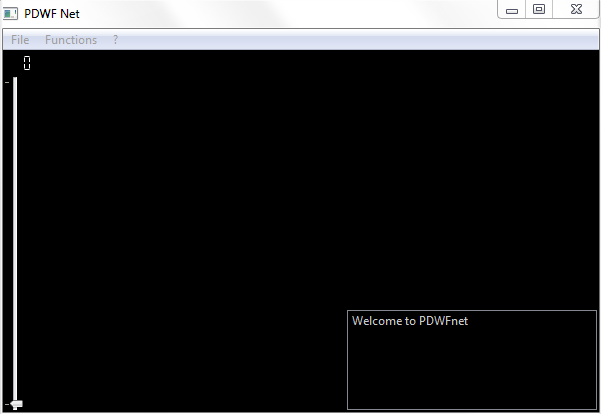
\includegraphics[width=.7\textwidth]{InitialInterface}

\subsection{The Basics}

An example, simple use of the program to load DICOM images and segment them is as follows:

\begin{enumerate}
	\item Run 'PDWFnet.exe'
	\item Select 'File$\rightarrow$ Import Images...' or press `Ctrl + I'. Other keyboard shortcuts are indicated next to menubar items.
	\item Click `Select Water Dicom Images...'
	\item Navigate to the directory of your DICOM files for water images
	\item Select the first DICOM file of the sequence and click 'Open'
	\item Repeat steps 3-5, except using `Select Fat Dicom Images...'
	\item Click `Import Selected Images'
	\item Upon finishing import, images will appear and can be viewed using the scroll wheel or click and dragging with left mouse button
	\item A segmentation model must be loaded. Select `File$\rightarrow$Load Model...'
	\item Navigate to the `Models' directory and select `SampleModel.hdf5'
	\item The images must be formatted to run the segmentation. Select `Functions$\rightarrow$Prepare Inputs'
	\item Start the segmentation by selecting `Functions$\rightarrow$Segment'
	\item After the segmentation has completed, you can select `View$\rightarrow$ Open Viewer' to visually examine all aspects of the segmentation.
	\item To correct errors, select `Functions$\rightarrow$Correct Segmentation'
	\item When you are satisfied with the mask, select 'File$\rightarrow$Save Data...' which will prompt for a location to save the PDWFnet output file as a MAT
	\item Once the data is saved, it may be reloaded using 'File$\rightarrow$Load Data...' to review the aspects of the segmentation or make changes

\end{enumerate}

%%%%%%%%%%%%%%%%%%%%%%%%%%%%%%%%%%%%%%%%%%%%%%%%%%%%%%%%%%%%%%%%%%%%

\section{Images}

\subsection{Image Format}

PDWFnet is currently designed to accept axial fat/water images in the form of a sequence of DICOMs. Additionally, preloaded DICOM sequences may be saved as .MAT files and imported that way as well.

For DICOM files, fat and water images should be stored alone in separate directories. All images in the sequence defined by the first image in the directory will be loaded as the image volume.

For MAT files, store each fat and water image volume in the same file as separate variables. PDWFnet will load 3D arrays of doubles or uint8/16. If the values are complex, their magnitude will be taken.

In order to conduct batch processing, images must be stored as separate variables in the same MAT file, with the series of MAT files stored in the same directory, like below.

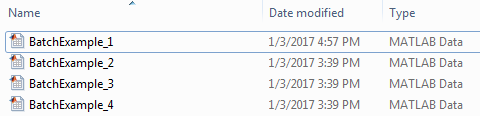
\includegraphics[width=.7\textwidth]{BatchMAT_cap.PNG}

In the example above, each BatchExample.mat file should have a water images variable and a fat images variable. Additionally, a complex version of each can be included in the import and final processing.

\subsection{Importing Images}

Once your images are ready for import, run PDWFnet and select `File$\rightarrow$Import Images...'. The following importing interface will appear.

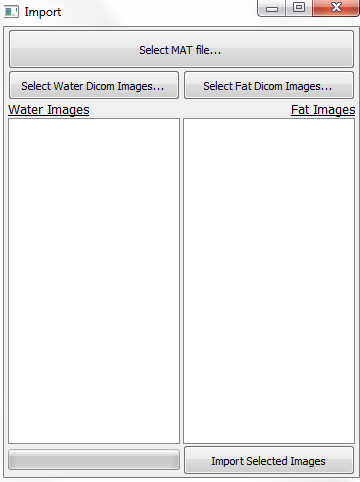
\includegraphics[width=.7\textwidth]{ImportGUI.PNG}

If you are importing a .MAT file, click `Select MAT file...' and navigate to the file containing the images you wish to import. The variables in the .MAT file will be displayed in each column. Select the variable in each column that corresponds to the type of images (Water/Fat).

If you are importing DICOM images, click `Select Water Dicom Images...' and nagivate to the directory of the images you wish to import. Select any image in the directory and click `Open'; the list of Dicom images in that directory will be displayed. Repeat the selection for Fat images.

At this time, both fat and water images must be loaded. In the future, this requirement will be updated to allow loading of a single volume.

The images you import will be saved in the PDWFnet output file, so using these images again can be done by using the load function rather than import.


\subsection{Loading Data}

Once you have imported images and run any calculation (or none at all), you may save the images into a formatted PDWF output .mat file. These files can then be loaded, rather than imported, using `File$\rightarrow$Load Data...'. All aspects of segmentation (excluding the model) will be reloaded to PDWFnet and will be accessible to view, redo, or correct.

\subsection{Save Data}

At any point after images are imported, you can generate a PDWFnet data file by selecting `File$\rightarrow$Save Data...'. You will be prompted to choose a location and filename for the data file. All pertinent aspects of the segmentation will be saved in a specifically formatted .mat file. This allows you to use the `Load Data' option rather than importing images.

\subsection{Load Model}

A Keras model will need to be loaded before segmenation can be performed. Select `File$\rightarrow$Load Model' and navigate to the Keras model you wish to use for segmentation, or use the included SampleModel.hdf5.

\subsection{Edit Preferences}

Select `File$\rightarrow$Edit Preferences...' to open a dialog that allows you to adjust various default settings of PDWFnet.


%%%%%%%%%%%%%%%%%%%%%%%%%%%%%%%%%%%%%%%%%%%%%%%%%%%%%%%%%%%%%%%%%%%%

\section{Functions}

%%%%%%%%%%%%%%%%%%%%%

\subsection{Shift Dimensions}

PDWFnet attempts to guess the relative dimensions of images imported from MAT files by assuming the smallest dimension of the array is the axial dimension. If this is not the case, the image display will be disconfigured and segmentation will not be performed properly. Correct the dimension order by selecting `Functions$\rightarrow$Shift Dimensions'. This may need to be selected twice to achieve the correct dimension ordering. If the axial plane is displayed in the largest frame, the dimension ordering is correct.

\subsection{Prepare Inputs}

Images need to be adjusted before they can be used as inputs for the Keras model. After importing water and fat images, select `Functions\ra Prepare Inputs'.

\subsection{Segment}

After images are imported, a Keras model is loaded, and inputs have been prepared, select `Functions\ra Segment' to perform the segmentation. Note that this process will run faster if more system memory is available to PDWFnet. It is recommended to close as many background programs as possible before running the segmenation.
The segmentation can take several seconds per slice when run on a CPU, and as fast as 0.03 seconds per slice when run on a high end GPU.

\subsection{Correct Segmentation}

Selecting `Functions\ra Correct Segmentation...' opens a separate window for making manual corrections to the segmentation mask. Further details are described in that \hyperref[Corrections]{section}.

\subsection{PDWF Calculations}
The \% FT (Fibroglandular Tissue- Breast density) can be calculated after segmentation, and additionally compared with the result after corrections are made. Select `Functions\ra Calculate PDWF' and the results will be printed in the display in the lower right corner.

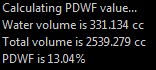
\includegraphics[width=.3\textwidth]{PDWFtable}.

The PDWF for each voxel is calculated by 
\begin{equation}
	WF = \frac{SI_w}{SI_w + SI_f}
\end{equation}
where $SI_w$ and $SI_f$ are the signal intensities of the corresponding water and fat voxels, respectively.The overall \% FT is calculated by summing $WF$ over the entire segmentation mask, divided by the total volume of the segmentation mask. Volumes are converted to cubic centimeters using the spatial resolution known by PDWFnet. If Dicom images were imported originally, the spatial resolution is obtained from the header. If images were imported from a MAT file, the spatial resolution is guessed using the matrix size of the images along with the defalt field-of-view that can be adjusted using the preferences dialog.

%%%%%%%%%%%%%%%%%%%%%

\textbf{\LARGE{{THE FOLLOWING HAS NOT YET BEEN UPDATED TO APPLY TO PDWFnet}}}


%%%%%%%%%%%%%%%%%%%%%

\section{Corrections}
\label{Corrections}


Selecting `Functions\ra Correct Segmentation' will open the corrections interface which will appear like below.

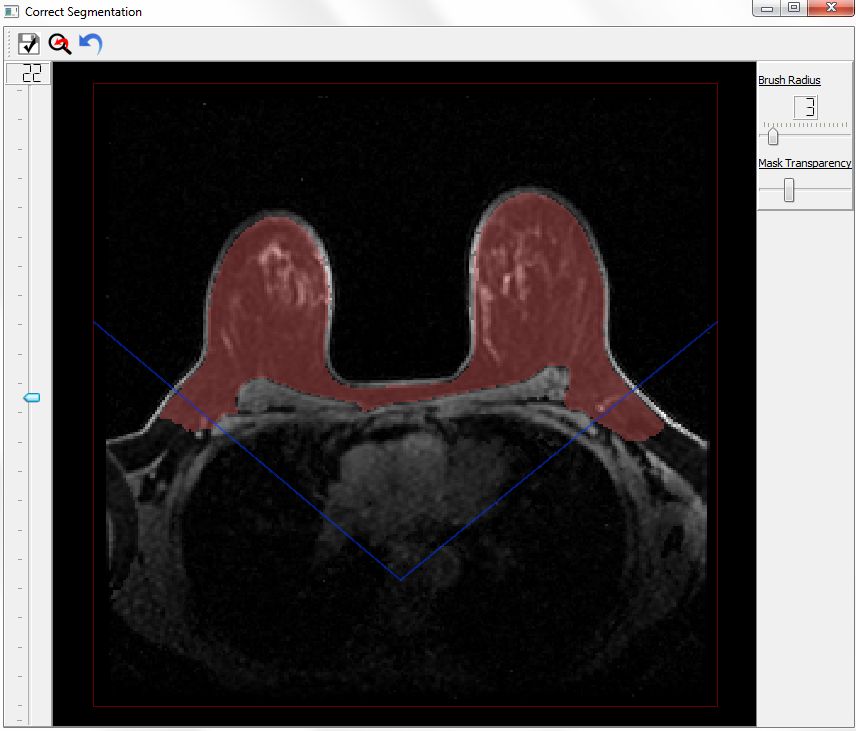
\includegraphics[width=1\textwidth]{CorrectionsGUI}\\

\subsection{User Interface}

\hspace{-1.6in}
\begin{minipage}{1.35\textwidth}
\normalsize{Each aspect of the corrections interface is described below}
\end{minipage}\\[1em]

\normalsize

\marginlabel{Slice Slider}
Slices can be scrolled through using the slider on the left, by moving the scroll wheel on your mouse, or by pressing the up/down arrows on your keyboard. The current slice number is indicated at the top of the slider. The top and bottom bounds are indicated on the left with red markers. Additionally, when either the top or bottom slice is active, a large red `B' or `T' will appear next to the slice number.

\marginlabel{Mask Overlay}
Toggle both the corrected and uncorrected segmentation mask overlays using the radio buttons on the right side of the interface. When both overlays are `On', the different regions of the mask are color-coded. Regions that are only part of the corrected mask are yellow, regions that are only part of the uncorrected mask are blue, and regions that are part of both masks are light green.

The corrected mask overlay can also be toggled by pressing `o' on your keyboard.

\marginlabel{Brush}
Use the dropdown below the mask toggles to select brush size to be used for corrections. The medium brush is selected by default. Note that due to limitations with MATLAB software, the actually footprint of the large brush is a circle that circumscribes the square cursor. For this reason, precise corrections are best done by the small and medium brush sizes.

Brush size can also be increased by pressing `period' (the `$>$' key) and decreased by  pressing `comma' (the`$<$' key).

\marginlabel{Message Box}
The textbox below the brush dropdown menu indicates whether the corrections you have made since the interface was opened are saved or not. Any error messages will also appear here.


\marginlabel{Reset Corrections}
The reset corrections button can be used to return the corrected mask to its original, uncorrected state. You will be asked for confirmation before the corrections are reset. Additionally, you will have to save the changes in the interface, and then save the data file in SegTrac in order to make the reset permanent. If corrections are reset inadvertently, simply close the corrections interface without saving changes.

\marginlabel{Correction Statistics}
After making each correction to the mask, the data displayed in the upper right corner of the interface will be updated.

\marginlabel{Toolbar}
The toolbar contains buttons for saving corrections, zooming and panning, and undo. Note that the undo button can only toggle undo/redo the last change that was made, and only applies to the slice that is currently active. For example, after making a correction and then shifting to the next slice, the undo button will not have any effect until a correction is made on the new slice.


The small and medium brushes will line up with the selection being made. The large brush is a circle, but due to limitations of MATLAB, the cursor will only appear as a large square.
Note that the cursors will not change size when zoom mode is activated, while the effective footprint increases by a factor of two. This means the brush and the cursor will no longer line up and the edge of the brush will have to be estimated based on the response of the GUI.



%%%

\subsection{Using the application}
Here are some tips to on how to properly use this application.


\marginlabel{Drawing}
Click and drag on the image to edit the displayed mask. Ctrl-click or right-click drag to erase. Drawing too quickly will result in a non-continuous line.

\index{Holes}\marginlabel{Holes}
The application does not allow holes in the mask. Any hole that would be made by either an addition or erasure from the mask will automatically be filled in. The application does allow the mask to be broken into multiple regions, but does eliminate isolated regions smaller than 10 pixels.



%%%
\subsection{Troubleshooting}

\index{Troubleshooting- Small bits}\marginlabel{Small bits of mask are disappearing}
Part of the processing of the mask after each edit is to remove tiny, standalone parts of the mask. This is designed to prevent unintended residue from erasing part of the mask. The application does not currently support any workaround. If this creates a problem in your use of the application, please contact \href{mailto:jmjohnson33@wisc.edu}{Jacob Johnson} and request a change.

\index{Troubleshooting- Disappear}\marginlabel{My selections are not doing anything}
There are two places where any selection you make will be ignored. The Vcut which defines the lateral boundaries of the mask is shown in red on all slices. The application does not support any selections outside of that boundary.
The mask processing also removes any holes from the mask. Thus, any selection while in erase mode that is completely within the current mask will be ignored, as it will create a hole that will be filled in.
If this behavior causes problems or there is other erroneous behavior, please inform \href{mailto:jmjohnson33@wisc.edu}{Jacob Johnson}.

\index{Troubleshooting-Undo}\marginlabel{The undo button doesn't do anything}
You only get 1 undo/redo! Additionally, the undo button only works on a per-slice basis. If you switch slices, the undo button will not do anything until you make a change to the current slice.


%%%%%%%%%%%%%%%%%%%%%





%%%%%%%%%%%%%%%%%%%%%%%%%%%%%%%%%%%%%%%%%%%%%%%%%%%%%%%%%%%%%%%%%%%%%%

\printindex

\end{document}
